\documentclass[11pt]{article}

\usepackage{amsmath}
\usepackage{amssymb}

\usepackage{graphicx}

\usepackage{ytableau}

\title{Matrices and graphs, \\ Math 4707, Spring 2021}
\date{}

\begin{document}





\maketitle


\vspace{-0.5cm}

\begin{enumerate}
\item Show that the number of closed walks of length $n$ in the complete graph $K_3$ on three vertices is $2^n+2\cdot(-1)^n$ by computing the eigenvalues of its adjacency matrix.
\item Explain how closed walks of length $n$ in $K_3$ are in bijection with words $w=(w_1,...,w_{n+1})$ of size $n+1$ in the alphabet $\{a,b,c\}$ for which $w_{i} \neq w_{i+1}$ for all $i=1,2,...,n$ and with $w_{n+1}=w_1$.
\item Explain how the words from the previous question are in bijection with ways to color the vertices of the cycle graph $C_n$ on $n$ vertices with three different colors so that adjacent vertices don't have the same color. These kind of graph colorings are usually called \emph{proper colorings}, or even just \emph{colorings} for short. Conclude that the number of proper 3-colorings of $C_n$ is $2^n+2\cdot(-1)^n$. 
\item Can you generalize the above to count proper $k$-colorings of $C_n$? {\bf Hint}: find the eigenvalues of the complete graph $K_k$ on $k$ vertices!
\end{enumerate}

\pagebreak

\begin{enumerate}
\setcounter{enumi}{4}
\item Find all the spanning trees of:
\[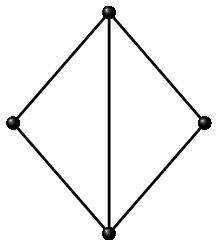
\includegraphics[width=1in]{kite.png}\]
\item Use the Matrix-Tree Theorem to count the spanning trees of the graph from the previous question.
\item The \emph{complete bipartite graph $K_{n,m}$} is the graph with vertex set $X\cup Y$ where $X=\{x_1,...,x_n\}$ and $Y=\{y_1,...,y_m\}$, and with edges $\{x_i,y_j\}$ for all $1\leq i \leq n, 1\leq j \leq m$ (but with no edges between the $x$'s, or between the $y$'s). Use the Matrix-Tree Theorem to show that the number of spanning trees of $K_{n,m}$ is $n^{m-1}m^{n-1}$. {\bf Hint}: you can use the fact from linear algebra that for a \emph{block matrix} $M$ of the form
\[ M=\begin{pmatrix} A & B \\ C & D \end{pmatrix}\]
we have $\mathrm{det}(M) = \mathrm{det}(A-BD^{-1}C)\mathrm{det}(D)$ as long as $D$ is invertible. (Observe that this is a generalization of the $2\times 2$ determinant formula $\mathrm{det}\begin{pmatrix}a & b \\ c & d\end{pmatrix} = ad-bc$.)
\end{enumerate}

%

\end{document}
